\documentclass[10.5pt]{article}
\def\examlang{ro}
\def\headyear{2026--2027}
% ===== Preambul comun pentru examen, banca de probleme și setul de exerciții (XeLaTeX) =====
% Statistica piețelor financiare / Statistics of Financial Markets -- Daniel Traian Pele
% Folosire: \documentclass[10.5pt]{article}  \def\examlang{ro} (sau en)  % ===== Preambul comun pentru examen, banca de probleme și setul de exerciții (XeLaTeX) =====
% Statistica piețelor financiare / Statistics of Financial Markets -- Daniel Traian Pele
% Folosire: \documentclass[10.5pt]{article}  \def\examlang{ro} (sau en)  % ===== Preambul comun pentru examen, banca de probleme și setul de exerciții (XeLaTeX) =====
% Statistica piețelor financiare / Statistics of Financial Markets -- Daniel Traian Pele
% Folosire: \documentclass[10.5pt]{article}  \def\examlang{ro} (sau en)  \input{../sfm_exam_preamble}
% Fișierele se compilează din exam/<subfolder>/, deci logo-urile sînt în ../../logos/.
\usepackage{fontspec}
\setmainfont{Helvetica Neue}
\usepackage{amsmath,amssymb}
\usepackage[a4paper,margin=1.9cm,top=2.4cm,headsep=0.5cm,headheight=14pt]{geometry}
\usepackage{graphicx}
\usepackage{float}
\usepackage{booktabs}
\usepackage{array}
\usepackage{enumitem}
\usepackage{xcolor}
\usepackage{fancyhdr}
\usepackage{lastpage}
\usepackage[hidelinks]{hyperref}
\definecolor{spfblue}{RGB}{26,58,110}
\definecolor{spfred}{RGB}{205,0,0}
\graphicspath{{../../logos/}{figs/}{../bank/figs/}{../practice/figs/}}

\providecommand{\examlang}{ro}
\newif\ifen
\def\tmpen{en}\ifx\examlang\tmpen\entrue\else\enfalse\fi

% etichete
\ifen
  \renewcommand{\figurename}{Figure}\renewcommand{\tablename}{Table}
  \newcommand{\coursetitle}{Statistics of Financial Markets}
  \newcommand{\subjword}{Problem}
  \newcommand{\rezword}{Solution.}
  \newcommand{\baremword}{Grading:}
\else
  \renewcommand{\figurename}{Figura}\renewcommand{\tablename}{Tabelul}
  \newcommand{\coursetitle}{Statistica piețelor financiare}
  \newcommand{\subjword}{Subiectul}
  \newcommand{\rezword}{Rezolvare.}
  \newcommand{\baremword}{Barem:}
\fi

% comutator: barem/rezolvare (true) sau subiecte (false)
\newif\ifrez \rezfalse

% antet / subsol
\pagestyle{fancy}
\fancyhf{}
\renewcommand{\headrulewidth}{0.4pt}
\lhead{\small\itshape \coursetitle}
\providecommand{\headyear}{2026}
\rhead{\small\bfseries \headyear}
\cfoot{\small\thepage/\pageref{LastPage}}

\setlength{\parindent}{0pt}
\setlength{\parskip}{0.42ex}
\setlength{\emergencystretch}{3em}

% numerotare automată, continuă, a cerințelor (1, 2, 3, ...)
\newcounter{qq}
\newcommand{\Q}{\refstepcounter{qq}\textbf{\theqq.}~}
% punctaj aliniat la dreapta, pe ultima linie a cerinței
\newcommand{\pts}[1]{\nobreak\hfill\textnormal{\itshape (#1)}\par}

% titlu de subiect: "Subiectul I • Titlu ........ puncte" + linie
\newcommand{\subiect}[3]{%
  \vspace{1.05ex}%
  {\color{spfblue}\bfseries \subjword\ #1 \textbullet\ #2}\hfill{\bfseries #3}\par
  \vspace{0.2ex}{\color{spfblue}\hrule height0.8pt}\vspace{0.7ex}}
% subiect numerotat automat (I, II, ...); argumentul opțional = identificatorul din bancă (vizibil doar în barem)
\newcounter{subj}
\newcommand{\problem}[3][]{%
  \stepcounter{subj}%
  \subiect{\Roman{subj}}{#2\ifrez\if\relax\detokenize{#1}\relax\else\ {\normalfont\footnotesize\color{spfred}[#1]}\fi\fi}{#3}}

% blocul de rezolvare (doar în barem)
\newcommand{\Rez}{\par\vspace{0.2ex}\textit{\rezword}\par\nopagebreak}
\newcommand{\barem}[1]{\par\textit{\baremword\ #1}\par}

% bloc de titlu cu sigle
\newcommand{\titlublock}[1]{%
\begin{center}
  \begin{minipage}[c]{0.16\textwidth}
\includegraphics[height=1.15cm]{ase_logo.png}\end{minipage}%
  \begin{minipage}[c]{0.68\textwidth}\centering
  \ifen
    {\bfseries Bucharest University of Economic Studies}\\[0.2ex]
    Faculty of Cybernetics, Statistics and Economic Informatics\\[0.2ex]
    Course: Statistics of Financial Markets
  \else
    {\bfseries Academia de Studii Economice din București}\\[0.2ex]
    Facultatea de Cibernetică, Statistică și Informatică Economică\\[0.2ex]
    Disciplina: Statistica piețelor financiare
  \fi
  \end{minipage}%
  \begin{minipage}[c]{0.16\textwidth}\raggedleft
\includegraphics[height=0.95cm]{ida_logo.png}\end{minipage}\\[1.2ex]
  {\large\bfseries #1}
\end{center}}

% valori utile generale (z_alpha = cuantila de ordin alpha a distribuției Normale standard)
\newcommand{\valoriutilegen}{%
\ifen Useful values: $z_{0.05}=-1.645$, $z_{0.025}=-1.960$, $z_{0.01}=-2.326$, $\varphi(1.960)=0.0584$,
$\varphi(2.326)=0.0267$, $\ln 2=0.693$, $\sqrt{252}\approx 15.87$, $\sqrt{365}\approx 19.10$,
$\chi^2_{0.95}(1)=3.84$, $\chi^2_{0.95}(2)=5.99$, $\chi^2_{0.95}(10)=18.31$
($z_p$ and $\chi^2_p$ are quantiles of order $p$; $\varphi$ is the standard Normal density).
\else Valori utile: $z_{0,05}=-1{,}645$; $z_{0,025}=-1{,}960$; $z_{0,01}=-2{,}326$; $\varphi(1{,}960)=0{,}0584$;
$\varphi(2{,}326)=0{,}0267$; $\ln 2=0{,}693$; $\sqrt{252}\approx 15{,}87$; $\sqrt{365}\approx 19{,}10$;
$\chi^2_{0,95}(1)=3{,}84$; $\chi^2_{0,95}(2)=5{,}99$; $\chi^2_{0,95}(10)=18{,}31$
($z_p$ și $\chi^2_p$ sînt cuantile de ordin $p$; $\varphi$ este densitatea distribuției Normale standard).\fi}

% titlul capitolului într-un fișier din bancă (folosit doar ca etichetă de build_variant.py)
\newcommand{\banktitle}[2]{}

% Fișierele se compilează din exam/<subfolder>/, deci logo-urile sînt în ../../logos/.
\usepackage{fontspec}
\setmainfont{Helvetica Neue}
\usepackage{amsmath,amssymb}
\usepackage[a4paper,margin=1.9cm,top=2.4cm,headsep=0.5cm,headheight=14pt]{geometry}
\usepackage{graphicx}
\usepackage{float}
\usepackage{booktabs}
\usepackage{array}
\usepackage{enumitem}
\usepackage{xcolor}
\usepackage{fancyhdr}
\usepackage{lastpage}
\usepackage[hidelinks]{hyperref}
\definecolor{spfblue}{RGB}{26,58,110}
\definecolor{spfred}{RGB}{205,0,0}
\graphicspath{{../../logos/}{figs/}{../bank/figs/}{../practice/figs/}}

\providecommand{\examlang}{ro}
\newif\ifen
\def\tmpen{en}\ifx\examlang\tmpen\entrue\else\enfalse\fi

% etichete
\ifen
  \renewcommand{\figurename}{Figure}\renewcommand{\tablename}{Table}
  \newcommand{\coursetitle}{Statistics of Financial Markets}
  \newcommand{\subjword}{Problem}
  \newcommand{\rezword}{Solution.}
  \newcommand{\baremword}{Grading:}
\else
  \renewcommand{\figurename}{Figura}\renewcommand{\tablename}{Tabelul}
  \newcommand{\coursetitle}{Statistica piețelor financiare}
  \newcommand{\subjword}{Subiectul}
  \newcommand{\rezword}{Rezolvare.}
  \newcommand{\baremword}{Barem:}
\fi

% comutator: barem/rezolvare (true) sau subiecte (false)
\newif\ifrez \rezfalse

% antet / subsol
\pagestyle{fancy}
\fancyhf{}
\renewcommand{\headrulewidth}{0.4pt}
\lhead{\small\itshape \coursetitle}
\providecommand{\headyear}{2026}
\rhead{\small\bfseries \headyear}
\cfoot{\small\thepage/\pageref{LastPage}}

\setlength{\parindent}{0pt}
\setlength{\parskip}{0.42ex}
\setlength{\emergencystretch}{3em}

% numerotare automată, continuă, a cerințelor (1, 2, 3, ...)
\newcounter{qq}
\newcommand{\Q}{\refstepcounter{qq}\textbf{\theqq.}~}
% punctaj aliniat la dreapta, pe ultima linie a cerinței
\newcommand{\pts}[1]{\nobreak\hfill\textnormal{\itshape (#1)}\par}

% titlu de subiect: "Subiectul I • Titlu ........ puncte" + linie
\newcommand{\subiect}[3]{%
  \vspace{1.05ex}%
  {\color{spfblue}\bfseries \subjword\ #1 \textbullet\ #2}\hfill{\bfseries #3}\par
  \vspace{0.2ex}{\color{spfblue}\hrule height0.8pt}\vspace{0.7ex}}
% subiect numerotat automat (I, II, ...); argumentul opțional = identificatorul din bancă (vizibil doar în barem)
\newcounter{subj}
\newcommand{\problem}[3][]{%
  \stepcounter{subj}%
  \subiect{\Roman{subj}}{#2\ifrez\if\relax\detokenize{#1}\relax\else\ {\normalfont\footnotesize\color{spfred}[#1]}\fi\fi}{#3}}

% blocul de rezolvare (doar în barem)
\newcommand{\Rez}{\par\vspace{0.2ex}\textit{\rezword}\par\nopagebreak}
\newcommand{\barem}[1]{\par\textit{\baremword\ #1}\par}

% bloc de titlu cu sigle
\newcommand{\titlublock}[1]{%
\begin{center}
  \begin{minipage}[c]{0.16\textwidth}
\includegraphics[height=1.15cm]{ase_logo.png}\end{minipage}%
  \begin{minipage}[c]{0.68\textwidth}\centering
  \ifen
    {\bfseries Bucharest University of Economic Studies}\\[0.2ex]
    Faculty of Cybernetics, Statistics and Economic Informatics\\[0.2ex]
    Course: Statistics of Financial Markets
  \else
    {\bfseries Academia de Studii Economice din București}\\[0.2ex]
    Facultatea de Cibernetică, Statistică și Informatică Economică\\[0.2ex]
    Disciplina: Statistica piețelor financiare
  \fi
  \end{minipage}%
  \begin{minipage}[c]{0.16\textwidth}\raggedleft
\includegraphics[height=0.95cm]{ida_logo.png}\end{minipage}\\[1.2ex]
  {\large\bfseries #1}
\end{center}}

% valori utile generale (z_alpha = cuantila de ordin alpha a distribuției Normale standard)
\newcommand{\valoriutilegen}{%
\ifen Useful values: $z_{0.05}=-1.645$, $z_{0.025}=-1.960$, $z_{0.01}=-2.326$, $\varphi(1.960)=0.0584$,
$\varphi(2.326)=0.0267$, $\ln 2=0.693$, $\sqrt{252}\approx 15.87$, $\sqrt{365}\approx 19.10$,
$\chi^2_{0.95}(1)=3.84$, $\chi^2_{0.95}(2)=5.99$, $\chi^2_{0.95}(10)=18.31$
($z_p$ and $\chi^2_p$ are quantiles of order $p$; $\varphi$ is the standard Normal density).
\else Valori utile: $z_{0,05}=-1{,}645$; $z_{0,025}=-1{,}960$; $z_{0,01}=-2{,}326$; $\varphi(1{,}960)=0{,}0584$;
$\varphi(2{,}326)=0{,}0267$; $\ln 2=0{,}693$; $\sqrt{252}\approx 15{,}87$; $\sqrt{365}\approx 19{,}10$;
$\chi^2_{0,95}(1)=3{,}84$; $\chi^2_{0,95}(2)=5{,}99$; $\chi^2_{0,95}(10)=18{,}31$
($z_p$ și $\chi^2_p$ sînt cuantile de ordin $p$; $\varphi$ este densitatea distribuției Normale standard).\fi}

% titlul capitolului într-un fișier din bancă (folosit doar ca etichetă de build_variant.py)
\newcommand{\banktitle}[2]{}

% Fișierele se compilează din exam/<subfolder>/, deci logo-urile sînt în ../../logos/.
\usepackage{fontspec}
\setmainfont{Helvetica Neue}
\usepackage{amsmath,amssymb}
\usepackage[a4paper,margin=1.9cm,top=2.4cm,headsep=0.5cm,headheight=14pt]{geometry}
\usepackage{graphicx}
\usepackage{float}
\usepackage{booktabs}
\usepackage{array}
\usepackage{enumitem}
\usepackage{xcolor}
\usepackage{fancyhdr}
\usepackage{lastpage}
\usepackage[hidelinks]{hyperref}
\definecolor{spfblue}{RGB}{26,58,110}
\definecolor{spfred}{RGB}{205,0,0}
\graphicspath{{../../logos/}{figs/}{../bank/figs/}{../practice/figs/}}

\providecommand{\examlang}{ro}
\newif\ifen
\def\tmpen{en}\ifx\examlang\tmpen\entrue\else\enfalse\fi

% etichete
\ifen
  \renewcommand{\figurename}{Figure}\renewcommand{\tablename}{Table}
  \newcommand{\coursetitle}{Statistics of Financial Markets}
  \newcommand{\subjword}{Problem}
  \newcommand{\rezword}{Solution.}
  \newcommand{\baremword}{Grading:}
\else
  \renewcommand{\figurename}{Figura}\renewcommand{\tablename}{Tabelul}
  \newcommand{\coursetitle}{Statistica piețelor financiare}
  \newcommand{\subjword}{Subiectul}
  \newcommand{\rezword}{Rezolvare.}
  \newcommand{\baremword}{Barem:}
\fi

% comutator: barem/rezolvare (true) sau subiecte (false)
\newif\ifrez \rezfalse

% antet / subsol
\pagestyle{fancy}
\fancyhf{}
\renewcommand{\headrulewidth}{0.4pt}
\lhead{\small\itshape \coursetitle}
\providecommand{\headyear}{2026}
\rhead{\small\bfseries \headyear}
\cfoot{\small\thepage/\pageref{LastPage}}

\setlength{\parindent}{0pt}
\setlength{\parskip}{0.42ex}
\setlength{\emergencystretch}{3em}

% numerotare automată, continuă, a cerințelor (1, 2, 3, ...)
\newcounter{qq}
\newcommand{\Q}{\refstepcounter{qq}\textbf{\theqq.}~}
% punctaj aliniat la dreapta, pe ultima linie a cerinței
\newcommand{\pts}[1]{\nobreak\hfill\textnormal{\itshape (#1)}\par}

% titlu de subiect: "Subiectul I • Titlu ........ puncte" + linie
\newcommand{\subiect}[3]{%
  \vspace{1.05ex}%
  {\color{spfblue}\bfseries \subjword\ #1 \textbullet\ #2}\hfill{\bfseries #3}\par
  \vspace{0.2ex}{\color{spfblue}\hrule height0.8pt}\vspace{0.7ex}}
% subiect numerotat automat (I, II, ...); argumentul opțional = identificatorul din bancă (vizibil doar în barem)
\newcounter{subj}
\newcommand{\problem}[3][]{%
  \stepcounter{subj}%
  \subiect{\Roman{subj}}{#2\ifrez\if\relax\detokenize{#1}\relax\else\ {\normalfont\footnotesize\color{spfred}[#1]}\fi\fi}{#3}}

% blocul de rezolvare (doar în barem)
\newcommand{\Rez}{\par\vspace{0.2ex}\textit{\rezword}\par\nopagebreak}
\newcommand{\barem}[1]{\par\textit{\baremword\ #1}\par}

% bloc de titlu cu sigle
\newcommand{\titlublock}[1]{%
\begin{center}
  \begin{minipage}[c]{0.16\textwidth}
\includegraphics[height=1.15cm]{ase_logo.png}\end{minipage}%
  \begin{minipage}[c]{0.68\textwidth}\centering
  \ifen
    {\bfseries Bucharest University of Economic Studies}\\[0.2ex]
    Faculty of Cybernetics, Statistics and Economic Informatics\\[0.2ex]
    Course: Statistics of Financial Markets
  \else
    {\bfseries Academia de Studii Economice din București}\\[0.2ex]
    Facultatea de Cibernetică, Statistică și Informatică Economică\\[0.2ex]
    Disciplina: Statistica piețelor financiare
  \fi
  \end{minipage}%
  \begin{minipage}[c]{0.16\textwidth}\raggedleft
\includegraphics[height=0.95cm]{ida_logo.png}\end{minipage}\\[1.2ex]
  {\large\bfseries #1}
\end{center}}

% valori utile generale (z_alpha = cuantila de ordin alpha a distribuției Normale standard)
\newcommand{\valoriutilegen}{%
\ifen Useful values: $z_{0.05}=-1.645$, $z_{0.025}=-1.960$, $z_{0.01}=-2.326$, $\varphi(1.960)=0.0584$,
$\varphi(2.326)=0.0267$, $\ln 2=0.693$, $\sqrt{252}\approx 15.87$, $\sqrt{365}\approx 19.10$,
$\chi^2_{0.95}(1)=3.84$, $\chi^2_{0.95}(2)=5.99$, $\chi^2_{0.95}(10)=18.31$
($z_p$ and $\chi^2_p$ are quantiles of order $p$; $\varphi$ is the standard Normal density).
\else Valori utile: $z_{0,05}=-1{,}645$; $z_{0,025}=-1{,}960$; $z_{0,01}=-2{,}326$; $\varphi(1{,}960)=0{,}0584$;
$\varphi(2{,}326)=0{,}0267$; $\ln 2=0{,}693$; $\sqrt{252}\approx 15{,}87$; $\sqrt{365}\approx 19{,}10$;
$\chi^2_{0,95}(1)=3{,}84$; $\chi^2_{0,95}(2)=5{,}99$; $\chi^2_{0,95}(10)=18{,}31$
($z_p$ și $\chi^2_p$ sînt cuantile de ordin $p$; $\varphi$ este densitatea distribuției Normale standard).\fi}

% titlul capitolului într-un fișier din bancă (folosit doar ca etichetă de build_variant.py)
\newcommand{\banktitle}[2]{}

\renewcommand{\subjword}{Problema}
\newcommand{\pp}[1]{\stepcounter{subj}\subiect{\arabic{subj}}{#1}{}}
\newcommand{\capitol}[1]{\par\vspace{1.4ex}{\large\bfseries\color{spfred}#1}\par\vspace{0.4ex}}
\setlist[enumerate]{label=(\alph*),leftmargin=2.2em,itemsep=0.15ex,topsep=0.3ex}
\begin{document}
\titlublock{PROBLEME DE EXAMEN --- SET DE EXERCIȚII}

\noindent Problemele au forma subiectelor de examen: un calcul scurt, urmat de interpretarea rezultatului.
Datele provin din seriile zilnice folosite la curs (ultima zi: 18 septembrie 2026). Răspunsurile numerice
sînt la sfîrșitul documentului.
Notații: $R_t$ randamentul simplu, $r_t=\ln(P_t/P_{t-1})$ randamentul logaritmic,
$\mathrm{VaR}_\alpha=-q_\alpha$ (VaR 1\% este pierderea depășită în 1\% din zile).\par
\vspace{0.4ex}{\small\noindent\valoriutilegen\par}

% ===================================================================================================
\capitol{Capitolul 1. Date, randamente și indicatori}

\pp{Randamentul unui portofoliu: Banca Transilvania și OMV Petrom în 2025}
Prețurile ajustate de închidere au fost $17{,}71$ lei (31 decembrie 2024) și $25{,}52$ de lei (31 decembrie 2025)
pentru Banca Transilvania (TLV), respectiv $0{,}615$ lei și $0{,}941$ lei pentru OMV Petrom (SNP). Un investitor a
cumpărat la 31 decembrie 2024 un portofoliu cu ponderile $60\%$ TLV și $40\%$ SNP, pe care l-a păstrat tot anul.
\begin{enumerate}
\item Calculați randamentul simplu al fiecărei acțiuni în 2025.
\item Calculați randamentul simplu al portofoliului.
\item Comparați randamentul logaritmic al portofoliului cu media ponderată a randamentelor logaritmice ale
celor două acțiuni.
\item Explicați de ce, pentru portofolii, se agregă randamentele simple, iar în timp randamentele logaritmice.
\end{enumerate}

\pp{Drawdown-ul indicelui BET în 2020}
Figura~\ref{fig:bet} arată indicele BET și drawdown-ul lui între 2015 și 2026. Vîrful dinaintea crahului
COVID-19 a fost $10\,219{,}75$ puncte (23 ianuarie 2020), minimul a fost $7\,038{,}95$ de puncte (23 martie 2020),
iar indicele a revenit la nivelul vîrfului pe 13 ianuarie 2021.
\begin{figure}[H]\centering
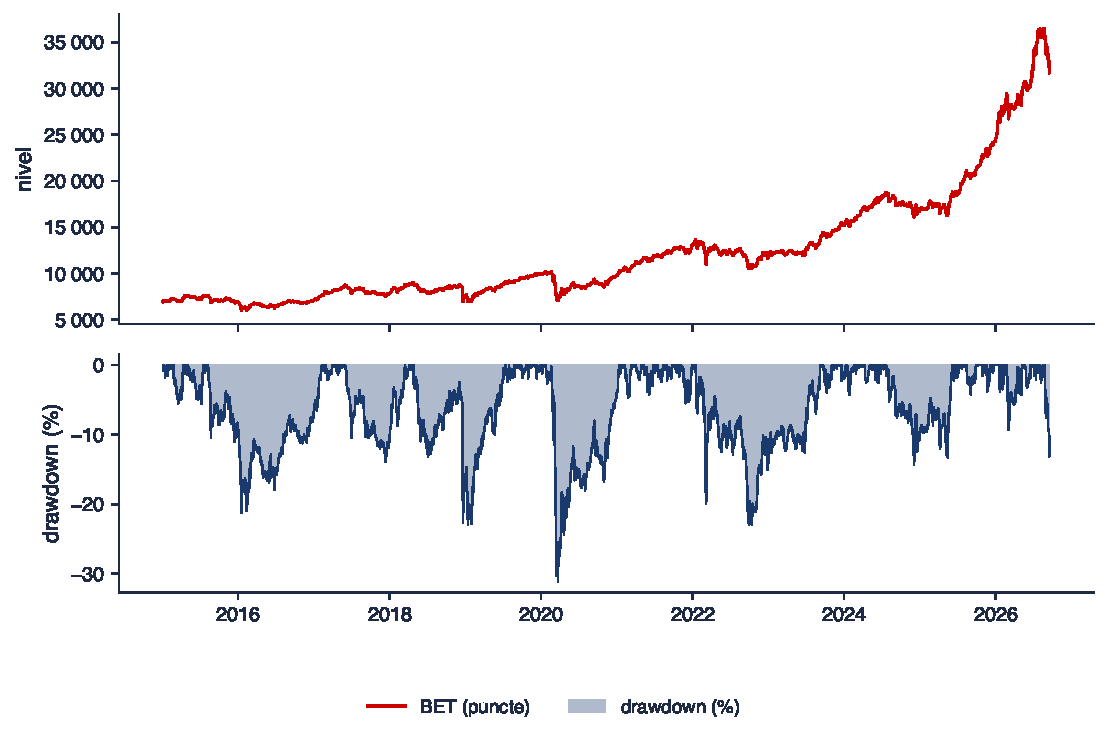
\includegraphics[width=0.66\textwidth]{practice_bet_drawdown_ro.pdf}
\caption{Indicele BET și drawdown-ul $D_t=P_t/\max_{s\le t}P_s-1$, 2015--2026.}\label{fig:bet}
\end{figure}
\begin{enumerate}
\item Calculați drawdown-ul maxim al episodului.
\item Calculați creșterea procentuală necesară pentru revenirea de la minim la vîrf.
\item Interpretați durata perioadei de sub vîrf (underwater) pentru un investitor cu orizont scurt.
\end{enumerate}

\pp{Raportul Sharpe și raportul Sortino: S\&P 500}
Pentru S\&P 500 (2015--2026, 252 de zile pe an), media anualizată a randamentelor logaritmice este $11{,}24\%$,
volatilitatea anualizată este $17{,}71\%$, iar semi-deviația negativă anualizată (pragul $\tau=0$) este
$\sigma_D=12{,}82\%$. Se consideră $r_f=0$.
\begin{enumerate}
\item Calculați raportul Sharpe.
\item Calculați raportul Sortino.
\item Explicați de ce raportul Sortino este mai mare decît raportul Sharpe pentru această serie.
\end{enumerate}

% ===================================================================================================
\capitol{Capitolul 2. Distribuții clasice și fapte stilizate}

\pp{Testul Jarque--Bera pentru DAX}
Pentru randamentele logaritmice zilnice ale indicelui DAX (2015--2026) s-au obținut $n=2972$, asimetria
$S=-0{,}565$ și excesul de boltire $K=9{,}973$.
\begin{enumerate}
\item Calculați statistica $\mathrm{JB}=\frac{n}{6}\left(S^2+K^2/4\right)$.
\item Calculați contribuția asimetriei și contribuția boltirii la statistica JB.
\item Formulați decizia testului la nivelul de semnificație de 5\%.
\end{enumerate}

\pp{Gaussianitatea agregată: S\&P 500}
Pentru randamentele logaritmice ale S\&P 500 (2015--2026), excesul de boltire este $15{,}85$ pentru randamentele
zilnice ($n=2943$), $10{,}80$ pentru sumele pe blocuri de 5 zile ($n=588$) și $4{,}00$ pentru sumele pe blocuri de
21 de zile ($n=140$). Pe blocurile de 21 de zile, asimetria este $S=-1{,}10$.
\begin{enumerate}
\item Testați normalitatea randamentelor pe 21 de zile cu statistica Jarque--Bera, la nivelul de semnificație de 5\%.
\item Explicați de ce excesul de boltire scade cînd orizontul crește.
\item Determinați numărul de grade de libertate $\nu$ al distribuției Student-$t$ cu excesul de boltire
$6/(\nu-4)$ egal cu $4{,}00$.
\end{enumerate}

\pp{Cea mai proastă zi a indicelui BET}
Pe 19 decembrie 2018, indicele BET a scăzut cu $11{,}89\%$ (randament logaritmic). În perioada 2015--2026
($n=2925$ de zile), media randamentelor zilnice este $0{,}053\%$, iar abaterea standard este $0{,}983\%$.
În aceeași perioadă, 42 de zile au avut $|z_t|>3$, unde $z_t=(r_t-\bar r)/s$.
\begin{enumerate}
\item Calculați randamentul standardizat al zilei de 19 decembrie 2018.
\item Interpretați probabilitatea Normală $\Phi(-12{,}15)\approx 2{,}8\cdot 10^{-34}$ a unei astfel de zile.
\item Comparați numărul de zile cu $|z_t|>3$ cu numărul așteptat sub distribuția Normală
($P(|Z|>3)=0{,}0027$).
\end{enumerate}

% ===================================================================================================
\capitol{Capitolul 3. Distribuții $\alpha$-stabile}

\pp{Momente și cozi pentru o lege stabilă}
Randamentele zilnice ale unui activ urmează o distribuție $\alpha$-stabilă cu $\alpha=1{,}5$. Pentru un prag $x$ mare,
$P(X>x)\approx C\,x^{-\alpha}$.
\begin{enumerate}
\item Precizați dacă media și varianța distribuției sînt finite.
\item Calculați raportul $P(X>2x)/P(X>x)$.
\item Calculați raportul $P(X>10x)/P(X>x)$.
\end{enumerate}

\pp{Metoda cuantilelor a lui McCulloch: BET}
Pentru randamentele logaritmice zilnice ale indicelui BET (2015--2026), cuantilele empirice (în \%) sînt
$q_{0,05}=-1{,}383$; $q_{0,25}=-0{,}380$; $q_{0,50}=0{,}085$; $q_{0,75}=0{,}543$; $q_{0,95}=1{,}417$.
\begin{enumerate}
\item Calculați $\nu_\alpha=(q_{0,95}-q_{0,05})/(q_{0,75}-q_{0,25})$.
\item Calculați $\nu_\beta=(q_{0,95}+q_{0,05}-2q_{0,5})/(q_{0,95}-q_{0,05})$.
\item Interpretați diferența dintre $\nu_\alpha$ și valoarea $2{,}44$ a distribuției Normale.
\end{enumerate}

% ===================================================================================================
\capitol{Capitolul 4. Probabilitate}

\pp{Diversificare: BET și S\&P 500}
Abaterile standard ale randamentelor zilnice sînt $0{,}983\%$ pentru BET și $1{,}116\%$ pentru S\&P 500
(2015--2026, zilele comune), iar corelația dintre ele este $\rho=0{,}305$.
\begin{enumerate}
\item Calculați abaterea standard zilnică a portofoliului cu ponderile $50\%$ și $50\%$.
\item Calculați raportul dintre această abatere standard și media ponderată a celor două abateri standard.
\item Calculați volatilitatea anualizată a portofoliului (252 de zile).
\end{enumerate}

\pp{Procesul AR(1): S\&P 500}
Autocorelația de ordinul 1 a randamentelor zilnice S\&P 500 (2015--2026) este $-0{,}13$. Randamentele sînt
modelate prin procesul AR(1) $X_t=\phi X_{t-1}+\varepsilon_t$, cu $\phi=-0{,}13$ și $\mathrm{Var}(\varepsilon_t)=\sigma^2$.
\begin{enumerate}
\item Calculați autocorelația de ordinul 2.
\item Calculați raportul $\mathrm{Var}(X_t)/\sigma^2$.
\item Propuneți o explicație pentru o autocorelație negativă de ordinul 1 la un indice bursier.
\end{enumerate}

% ===================================================================================================
\capitol{Capitolul 5. Cozi groase și teoria valorilor extreme}

\pp{Hill plot pentru Bitcoin}
Figura~\ref{fig:hill} arată estimatorul Hill $\hat\alpha_k$ al indicelui de coadă pentru pierderile zilnice ale
Bitcoin (2015--2026, $n=4278$), în funcție de numărul $k$ de pierderi folosite. Pentru $k=100$, $\hat\alpha=2{,}69$.
\begin{figure}[H]\centering
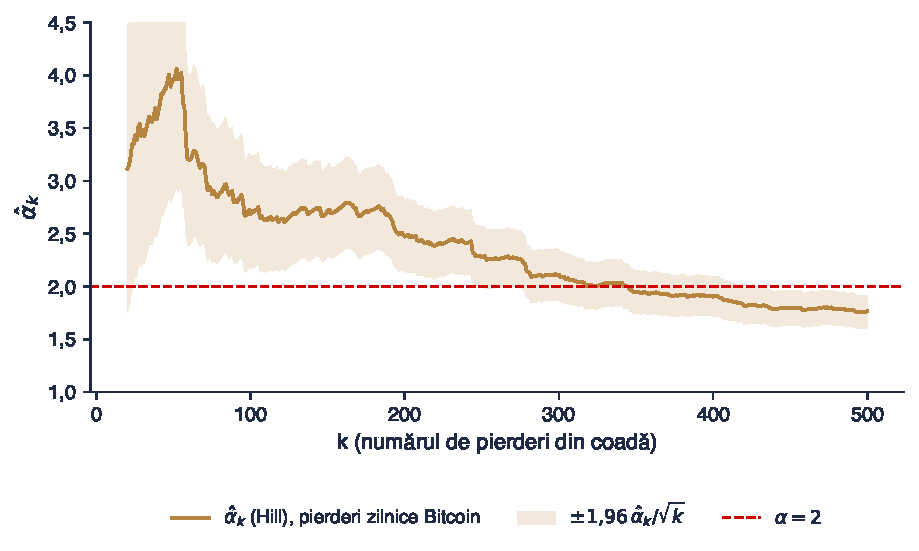
\includegraphics[width=0.62\textwidth]{practice_btc_hill_ro.pdf}
\caption{Hill plot: pierderile zilnice ale Bitcoin, 2015--2026.}\label{fig:hill}
\end{figure}
\begin{enumerate}
\item Calculați eroarea standard $\hat\alpha/\sqrt{k}$ și intervalul de încredere de 95\% pentru $k=100$.
\item Precizați dacă, pe baza acestui interval, varianța pierderilor este finită.
\item Explicați de ce estimările pentru $k=50$ ($3{,}96$) și $k=400$ ($1{,}90$) diferă atît de mult.
\end{enumerate}

\pp{O coadă Pareto pentru S\&P 500}
Pentru pierderile zilnice ale S\&P 500 (2015--2026, în \%), dreapta estimată pe graficul log--log al cozii este
$\ln\hat P(L>x)=-1{,}391-2{,}753\ln x$.
\begin{enumerate}
\item Calculați probabilitatea unei pierderi zilnice mai mari de 7\%.
\item Exprimați rezultatul de la punctul (a) ca perioadă medie de revenire, în ani de 252 de zile.
\item Precizați dacă varianța pierderilor este finită pentru acest indice de coadă.
\end{enumerate}

% ===================================================================================================
\capitol{Capitolul 6. Selecția modelului și managementul riscului}

\pp{Distribuția Normală sau distribuția Student-$t$ pentru Bitcoin?}
Pe $n=4278$ de randamente zilnice ale Bitcoin (2015--2026), log-verosimilitatea maximă este $\ell_N=-11\,415{,}1$
pentru distribuția Normală (2 parametri) și $\ell_t=-10\,745{,}8$ pentru distribuția Student-$t$ cu poziție și scală
(3 parametri, $\hat\nu=2{,}19$). Se dă $\ln 4278=8{,}36$.
\begin{enumerate}
\item Calculați AIC pentru cele două modele.
\item Calculați BIC pentru cele două modele.
\item Precizați ce implică $\hat\nu=2{,}19$ pentru existența boltirii.
\end{enumerate}

\pp{Testul Kupiec}
Un model VaR 1\% înregistrează $x=11$ excepții în $n=500$ de zile.
\begin{enumerate}
\item Calculați rata empirică a excepțiilor.
\item Calculați statistica $LR_{uc}=-2\ln\dfrac{(1-\alpha)^{n-x}\alpha^x}{(1-\hat\pi)^{n-x}\hat\pi^x}$, cu $\hat\pi=x/n$.
\item Formulați decizia la nivelul de semnificație de 5\%.
\end{enumerate}

% ===================================================================================================
\capitol{Capitolul 7. Ipoteza piețelor eficiente, mersul aleator și testele VR}

\pp{Autocorelațiile randamentelor și ale randamentelor absolute: S\&P 500}
Figura~\ref{fig:acf} arată autocorelațiile randamentelor zilnice S\&P 500 și ale randamentelor absolute
(2015--2026, $n=2943$). Primele cinci autocorelații ale randamentelor sînt $-0{,}128$; $0{,}078$; $-0{,}031$;
$-0{,}062$; $0{,}047$.
\begin{figure}[H]\centering
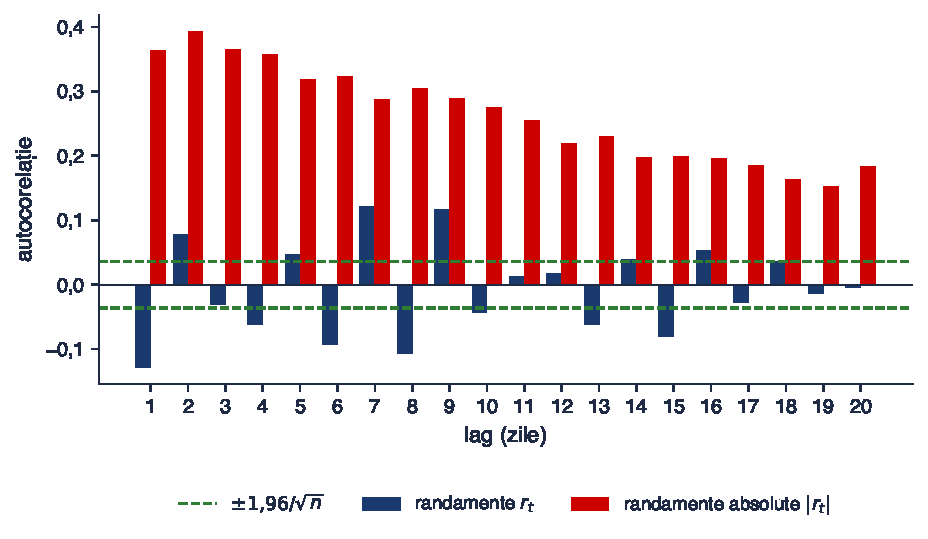
\includegraphics[width=0.62\textwidth]{practice_sp500_acf_ro.pdf}
\caption{ACF pentru $r_t$ și $|r_t|$, S\&P 500, 2015--2026.}\label{fig:acf}
\end{figure}
\begin{enumerate}
\item Calculați limitele benzii $\pm 1{,}96/\sqrt n$.
\item Precizați cîte dintre primele cinci autocorelații ale randamentelor ies din bandă.
\item Interpretați diferența dintre autocorelațiile lui $r_t$ și cele ale lui $|r_t|$.
\end{enumerate}

\pp{Raportul varianțelor din autocorelații: DAX}
Pentru DAX (2015--2026, $T=2972$), primele patru autocorelații ale randamentelor zilnice sînt $-0{,}020$; $0{,}034$;
$0{,}014$; $-0{,}014$. Sub ipoteza de mers aleator cu varianță constantă, abaterea standard a lui
$\widehat{\mathrm{VR}}(5)$ este $0{,}0402$.
\begin{enumerate}
\item Calculați $\mathrm{VR}(5)=1+2\sum_{k=1}^{4}(1-k/5)\hat\rho(k)$.
\item Testați ipoteza de mers aleator la nivelul de 5\%, cu statistica $z=(\mathrm{VR}(5)-1)/0{,}0402$.
\item Interpretați rezultatul din perspectiva eficienței în formă slabă.
\end{enumerate}

% ===================================================================================================
\capitol{Capitolul 8. Estimatori de volatilitate}

\pp{Estimatori de amplitudine: S\&P 500 pe 9 aprilie 2025}
Pe 9 aprilie 2025 (ziua anunțării suspendării unor tarife vamale), S\&P 500 a avut $O=4965{,}28$;
$H=5481{,}34$; $L=4948{,}43$; $C=5456{,}90$, iar închiderea din ziua anterioară a fost $4982{,}77$.
Notații: $u=\ln(H/O)$, $d=\ln(L/O)$, $c=\ln(C/O)$.
\begin{enumerate}
\item Calculați varianța Parkinson $(u-d)^2/(4\ln 2)$ și volatilitatea zilnică corespunzătoare.
\item Calculați varianța Garman--Klass $0{,}5(u-d)^2-(2\ln 2-1)c^2$ și volatilitatea zilnică corespunzătoare.
\item Explicați de ce estimatorul Garman--Klass dă o valoare mai mică într-o zi cu o tendință puternică.
\end{enumerate}

\pp{O actualizare EWMA}
Volatilitatea zilnică estimată ieri prin EWMA era $1{,}2\%$, iar randamentul de ieri a fost $-3{,}5\%$.
\begin{enumerate}
\item Calculați volatilitatea de azi pentru $\lambda=0{,}94$ (RiskMetrics).
\item Calculați timpul de înjumătățire al ponderilor, $\ln 0{,}5/\ln\lambda$, pentru $\lambda=0{,}94$ și pentru
$\lambda=0{,}97$.
\item Precizați care dintre cele două valori ale lui $\lambda$ reacționează mai repede la șocuri.
\end{enumerate}

% ===================================================================================================
\capitol{Capitolul 9. Modele ARCH și GARCH}

\pp{GARCH(1,1)-$t$ pentru BET}
Modelul GARCH(1,1) cu inovații Student-$t$ estimat pe randamentele zilnice ale BET (în \%, 2015--2026) are
$\hat\omega=0{,}0691$; $\hat\alpha=0{,}1846$; $\hat\beta=0{,}7401$.
\begin{enumerate}
\item Calculați persistența $\alpha+\beta$.
\item Calculați varianța de lungă durată și volatilitatea anualizată corespunzătoare (252 de zile).
\item Calculați timpul de înjumătățire al unui șoc de volatilitate.
\end{enumerate}

\pp{Prognoza volatilității pe mai mulți pași}
Cu parametrii din problema anterioară, varianța condiționată pentru mîine este $\sigma^2_{t+1}=4$ (volatilitate
de 2\%).
\begin{enumerate}
\item Calculați prognoza $E_t[\sigma^2_{t+10}]=\bar\sigma^2+(\alpha+\beta)^{9}(\sigma^2_{t+1}-\bar\sigma^2)$.
\item Calculați volatilitatea pe 10 zile ca rădăcina sumei prognozelor $E_t[\sigma^2_{t+h}]$, $h=1,\dots,10$.
\item Comparați rezultatul cu regula $\sqrt{10}\,\sigma_{t+1}$.
\end{enumerate}

% ===================================================================================================
\capitol{Capitolul 10. VaR, ES și backtesting}

\pp{VaR și ES pentru Banca Transilvania}
Pentru randamentele logaritmice zilnice ale acțiunii Banca Transilvania (2015--2026), media este $0{,}106\%$, iar
abaterea standard este $1{,}685\%$. Simularea istorică dă VaR 1\% $=4{,}58\%$ și ES 2,5\% $=4{,}93\%$.
\begin{enumerate}
\item Calculați VaR 1\% și ES 2,5\% sub distribuția Normală, cu $\mathrm{ES}_\alpha=-\mu+\sigma\varphi(z_\alpha)/\alpha$.
\item Exprimați VaR 1\% istoric în lei pentru o poziție de $50\,000$ de lei, cu formula $W(1-e^{-\mathrm{VaR}/100})$.
\item Explicați diferența dintre rezultatele celor două metode.
\end{enumerate}

\pp{Gruparea excepțiilor: testul Christoffersen}
Un model VaR 1\% are 10 excepții în 500 de zile. Dintre cele 10 excepții, 3 au urmat imediat după o altă
excepție. Numerele de tranziții sînt: $n_{00}=482$; $n_{01}=7$; $n_{10}=7$; $n_{11}=3$ ($n_{ij}$: zile în starea $j$
precedate de o zi în starea $i$; 1 înseamnă excepție).
\begin{enumerate}
\item Calculați $\hat\pi_{01}=n_{01}/(n_{00}+n_{01})$.
\item Calculați $\hat\pi_{11}=n_{11}/(n_{10}+n_{11})$.
\item Formulați decizia testului de independență, știind că $LR_{ind}=12{,}43$.
\end{enumerate}

% ===================================================================================================
\capitol{Capitolul 11. Ipoteza piețelor fractale și memoria lungă}

\pp{Exponentul Hurst și scalarea riscului}
Statistica R/S medie a unei serii de randamente este $3{,}2$ pentru blocuri de $n=10$ zile și $42$ pentru blocuri
de $n=1000$ de zile.
\begin{enumerate}
\item Calculați exponentul Hurst ca pantă în coordonate log--log.
\item Calculați parametrul de memorie $d=H-0{,}5$ al modelului ARFIMA$(0,d,0)$ corespunzător.
\item Calculați VaR 1\% pe 20 de zile, pornind de la VaR 1\% zilnic de $2{,}5\%$, cu scalarea $h^{H}$ și cu
scalarea $\sqrt h$.
\end{enumerate}

% ===================================================================================================
\capitol{Capitolul 12. Modele de scoring}

\pp{Scorul Z al lui Altman}
O companie industrială listată are: capital de lucru/active totale $X_1=0{,}12$; rezultat reportat/active totale
$X_2=0{,}25$; EBIT/active totale $X_3=0{,}08$; valoarea de piață a capitalului propriu/datorii totale $X_4=0{,}60$;
vînzări/active totale $X_5=1{,}10$.
\begin{enumerate}
\item Calculați $Z=1{,}2X_1+1{,}4X_2+3{,}3X_3+0{,}6X_4+1{,}0X_5$.
\item Încadrați compania în zonele lui Altman ($Z<1{,}81$ zona de risc; $1{,}81\le Z\le 2{,}99$ zona gri;
$Z>2{,}99$ zona sigură).
\item Precizați variabila care contribuie cel mai mult la scor.
\end{enumerate}

% ===================================================================================================
\capitol{Capitolul 13. Învățare automată}

\pp{Pierderea cuantilică pentru două prognoze VaR}
Două modele prognozează cuantila de 5\% a randamentului zilnic: modelul A dă $q_A=-2\%$, iar modelul B dă
$q_B=-1{,}5\%$, în fiecare din 4 zile. Randamentele realizate au fost $1{,}0\%$; $-0{,}5\%$; $-2{,}5\%$; $0{,}8\%$.
Pierderea cuantilică este $\rho_\alpha(u)=u\,(\alpha-\mathbf 1\{u<0\})$, cu $u=r_t-q$ și $\alpha=0{,}05$.
\begin{enumerate}
\item Calculați pierderea cuantilică medie a modelului A.
\item Calculați pierderea cuantilică medie a modelului B.
\item Explicați de ce pierderea cuantilică, și nu eroarea pătratică, se folosește pentru compararea prognozelor VaR.
\end{enumerate}

% ===================================================================================================
\capitol{Capitolul 14. Active cripto}

\pp{Bitcoin în weekend}
Pentru Bitcoin (2015--2026), abaterea standard a randamentelor zilnice este $2{,}675\%$ în zilele de weekend și
$3{,}765\%$ în zilele lucrătoare. Un an are 104 zile de weekend și 261 de zile lucrătoare.
\begin{enumerate}
\item Calculați raportul dintre volatilitatea din weekend și cea din zilele lucrătoare.
\item Calculați ponderea zilelor de weekend în varianța anuală.
\item Explicați de ce weekendul este mai liniștit pe piața Bitcoin.
\end{enumerate}

% ===================================================================================================
\capitol{Capitolul 15. Risc sistemic}

\pp{Zile proaste comune: JPMorgan Chase și S\&P 500}
Pe $n=2932$ de zile comune (2015--2026), o „zi proastă” este o zi în care randamentul este sub propria cuantilă de
5\%. S\&P 500 a avut 147 de zile proaste, iar în 74 dintre ele și JPMorgan Chase a avut o zi proastă.
\begin{enumerate}
\item Calculați numărul de zile proaste comune așteptat dacă cele două serii ar fi independente.
\item Calculați probabilitatea condiționată $P(\text{zi proastă JPM}\mid\text{zi proastă S\&P 500})$.
\item Interpretați rezultatul din perspectiva riscului sistemic.
\end{enumerate}

% ===================================================================================================
\clearpage
\capitol{Răspunsuri}
{\small
\begin{enumerate}[label=\textbf{\arabic*.},leftmargin=2.2em,itemsep=0.25ex]
\item (a) TLV $44{,}10\%$; SNP $52{,}94\%$. (b) $47{,}64\%$. (c) $\ln(1{,}4764)=38{,}96\%$, față de media ponderată
$38{,}92\%$: randamentele logaritmice nu se agregă exact între active. (d) Randamentul simplu al portofoliului este
media ponderată a randamentelor simple; randamentele logaritmice se adună în timp.
\item (a) $-31{,}12\%$. (b) $+45{,}19\%$. (c) Aproape un an sub vîrf (ianuarie 2020 -- ianuarie 2021).
\item (a) $0{,}63$. (b) $0{,}88$. (c) Semi-deviația negativă este mai mică decît volatilitatea totală: o parte din
variabilitate provine din creșteri.
\item (a) $\mathrm{JB}\approx 12\,475$. (b) Asimetria $158$; boltirea $12\,317$ (aproape în întregime).
(c) $\mathrm{JB}\gg 5{,}99$: se respinge normalitatea.
\item (a) $\mathrm{JB}=121{,}7>5{,}99$: se respinge normalitatea și la orizontul de 21 de zile. (b) Suma mai
multor randamente se apropie de distribuția Normală (teorema limită centrală), dar lent, din cauza volatility
clustering. (c) $\nu=5{,}5$.
\item (a) $z=-12{,}15$. (b) Sub distribuția Normală, o astfel de zi ar apărea o dată la aproximativ $10^{31}$ ani:
modelul Normal subestimează grav cozile. (c) Așteptat $7{,}9$ zile, observat 42: de circa $5{,}3$ ori mai multe.
\item (a) Media este finită ($1<\alpha$); varianța este infinită ($2>\alpha$). (b) $2^{-1{,}5}=0{,}354$.
(c) $10^{-1{,}5}=0{,}032$; pentru distribuția Normală raportul este practic zero.
\item (a) $3{,}03$. (b) $-0{,}05$. (c) $3{,}03>2{,}44$: cozi mai groase decît la distribuția Normală
($\alpha<2$); $\nu_\beta\approx 0$ indică o distribuție aproape simetrică.
\item (a) $0{,}848\%$. (b) $0{,}81$: diversificarea reduce riscul cu circa 19\%. (c) $0{,}848\%\cdot\sqrt{252}=13{,}5\%$.
\item (a) $\phi^2=0{,}017$. (b) $1/(1-\phi^2)=1{,}017$. (c) Supra-reacția la știri corectată a doua zi; în cazul
acțiunilor individuale, și oscilația prețului între bid și ask.
\item (a) $\mathrm{SE}=0{,}27$; IC $[2{,}16;\ 3{,}22]$. (b) Da: intervalul este peste 2. (c) Pentru $k$ mic estimatorul
are varianță mare; pentru $k$ mare intră în calcul observații din centrul distribuției și apare deplasarea.
\item (a) $e^{-1{,}391}\cdot 7^{-2{,}753}=1{,}17\cdot 10^{-3}$. (b) Aproximativ 853 de zile, adică $3{,}4$ ani.
(c) Da: $\alpha=2{,}753>2$ (momentele de ordin mai mic decît $\alpha$ sînt finite).
\item (a) $22\,834{,}2$ și $21\,497{,}6$. (b) $22\,846{,}9$ și $21\,516{,}7$; ambele criterii aleg distribuția
Student-$t$. (c) $\nu\le 4$: boltirea (momentul de ordinul 4) este infinită, iar varianța există doar la limită
($\nu>2$).
\item (a) $2{,}2\%$. (b) $LR_{uc}=5{,}42$. (c) $5{,}42>3{,}84$: se respinge acoperirea corectă (prea multe excepții).
\item (a) $\pm 0{,}036$. (b) Patru ($-0{,}128$; $0{,}078$; $-0{,}062$; $0{,}047$). (c) Semnul randamentului este greu de
anticipat, mărimea lui nu: autocorelațiile lui $|r_t|$ sînt mari și scad lent (volatility clustering). Banda
presupune varianță constantă, deci pentru $r_t$ este prea îngustă.
\item (a) $1{,}014$. (b) $z=0{,}36<1{,}96$: nu se respinge mersul aleator. (c) Randamentele DAX pe 5 zile nu sînt
previzibile din randamentele trecute: rezultatul este compatibil cu eficiența în formă slabă.
\item (a) $3{,}77\cdot 10^{-3}$; $6{,}14\%$. (b) $1{,}79\cdot 10^{-3}$; $4{,}23\%$. (c) Termenul $-(2\ln 2-1)c^2$ scade
varianța cînd închiderea este aproape de maxim.
\item (a) $1{,}445\%$. (b) $11{,}2$ zile; $22{,}8$ zile. (c) $\lambda=0{,}94$.
\item (a) $0{,}925$. (b) $\bar\sigma^2=0{,}918$; $0{,}958\%$ pe zi; $15{,}2\%$ pe an. (c) $8{,}9$ zile.
\item (a) $2{,}44$ (volatilitate $1{,}56\%$). (b) $\sqrt{31{,}40}=5{,}60\%$. (c) $\sqrt{10}\cdot 2\%=6{,}32\%$:
regula supraestimează, pentru că volatilitatea revine la medie.
\item (a) VaR 1\% $=3{,}81\%$; ES 2,5\% $=3{,}83\%$. (b) $2236$ de lei. (c) Metoda istorică dă valori cu circa
$20\%$--$29\%$ mai mari: cozile groase nu sînt surprinse de distribuția Normală.
\item (a) $7/489=0{,}014$. (b) $3/10=0{,}30$. (c) $12{,}43>3{,}84$: se respinge independența; după o excepție,
probabilitatea unei noi excepții este de circa 20 de ori mai mare (modelul reacționează prea lent la volatilitate).
\item (a) $H=0{,}56$. (b) $d=0{,}06$. (c) $13{,}3\%$ cu $h^H$, față de $11{,}2\%$ cu $\sqrt h$.
\item (a) $Z=2{,}22$. (b) Zona gri. (c) $X_5$ (contribuție $1{,}10$).
\item (a) $(0{,}150+0{,}075+0{,}475+0{,}140)/4=0{,}21$. (b) $(0{,}125+0{,}050+0{,}950+0{,}115)/4=0{,}31$; modelul A
este mai bun. (c) Cuantila este minimizatorul pierderii cuantilice (VaR este elicitabil pentru această funcție);
eroarea pătratică evaluează media, nu cuantila.
\item (a) $0{,}71$. (b) $104\cdot 2{,}675^2/(104\cdot 2{,}675^2+261\cdot 3{,}765^2)=16{,}7\%$, deși weekendul are
$28{,}5\%$ din zile. (c) Piețele tradiționale sînt închise: lipsesc știrile macroeconomice, fluxurile instituționale
și arbitrajul cu ETF-urile.
\item (a) $2932\cdot 0{,}05^2=7{,}3$ zile (observat: 74, de circa 10 ori mai multe). (b) $74/147=0{,}50$, față de
$0{,}05$ fără condiționare. (c) Banca suferă împreună cu piața: diversificarea dispare tocmai în zilele proaste,
ceea ce măsoară $\Delta$CoVaR și MES.
\end{enumerate}}
\end{document}
